
\subsection{Equivalente eléctrico del calor}
Una resistencia en un circuito simple disipa energía siguiendo la relación

\begin{equation}
    \label{eq:energy_change_in_time}
    \frac{\Delta W}{\Delta t} = \frac{V^2}{R}
\end{equation}
Donde $V$ es la tensión y $R$ la resistencia eléctrica, esta razón es precisamente a la cual la resistencia, cuando está sumergida en algún líquido, le entrega energía al líquido, por ejemplo agua, en forma de calor.
Una cierta masa $m$ de agua sometida a un cambio de temperatura $\Delta T$ recibe una cantidad $\Delta Q$ de calor dada por la expresión

\begin{equation}
    \Delta Q = mc\,\Delta T, \label{eq:specific_differential_heat}
\end{equation}
donde $c$ es el calor específico del agua.

Si la variación de temperatura se da en función del tiempo, entonces:
\begin{equation}
    \frac{\Delta Q}{\Delta t} = mc \frac{\Delta T}{\Delta t}
    \label{eq:heat_change_in_time}
\end{equation}

Experimentalmente, se debe considerar el calor absorbido por vaso interno del calorímetro. 
\begin{equation}
    \frac{\Delta Q}{\Delta t} = (m + k)c \frac{\Delta T}{\Delta t}
    \label{eq:Q_dot_plus_calorimeter}
\end{equation}
Donde se ha definido $k=\dfrac{m_{\text{cal.}}c_{\text{cal.}}}{c_{\text{agua}}}$ la masa de agua equivalente del calorímetro.
Dividiendo la ecuación \eqref{eq:energy_change_in_time} por \eqref{eq:Q_dot_plus_calorimeter} se obtiene el equivalente eléctrico del calor. Para que esta cantidad se determine respecto a una diferencia de temperatura $\Delta T = \SI{1}{\celsius}$ se toma la ecuación \eqref{eq:Q_dot_plus_calorimeter} en unidades de $\si{\calorie\per\second}$, y teniendo en cuenta que la unidad caloría se deriva de la ecuación \eqref{eq:specific_differential_heat} con $c=1$ (para el mismo $\Delta T$), con la potencia eléctrica medida en $\si{\joule\per\second}$, se llega a que

\begin{equation}
    \label{eq:electrical_equivalent}
    J_{\text{elec.}}=\frac{\Delta W}{\Delta Q} = \dfrac{V^2}{R (m + k) (\Delta T / \Delta t)} 
    \quad \si{\joule\per\calorie}
\end{equation}
\subsection{Equivalente mecánico del calor}

La determinación del equivalente mecánico está ligada completamente al tipo de experimento que se realice, pues de este dependerá la naturaleza del trabajo mecánico. En el experimento particular que se realiza en el presente, se tiene la siguiente configuración (ver fig. \ref{fig:montaje_mec}): una polea con manivela que puede rotar aproximadamente sin fricción, a la que se le enrolla una cuerda que se fija en un de los extremos y en el otro se suspende una masa. El trabajo lo realiza entonces la fuerza de fricción que se da entre la cuerda y la polea.


\begin{figure}
    \begin{subfigure}{0.45\textwidth}
        \centering
        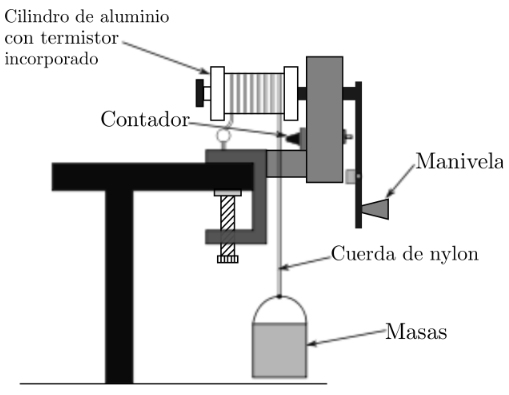
\includegraphics[width=0.85\linewidth]{img/montaje_mec.png}
        \caption{Montaje para el equivalente mecánica del calor}
        \label{fig:montaje_mec}
    \end{subfigure}
    \hfill
    \begin{subfigure}{0.45\textwidth}
        \centering
        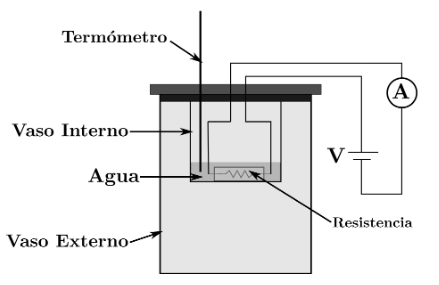
\includegraphics[width=0.85\linewidth]{img/esquema_elec.png}
        \caption{Montaje para hallar el equivalente eléctrico del calor}
        \label{fig:esquema_elec}
    \end{subfigure}
\end{figure}

La energía es entregada por cada vuelta que se le da la polea, por lo que para un número total de vueltas $n$ el trabajo total realizado será $W = \alpha n$, siendo $\alpha$ la cantidad de trabajo realizado por vuelta (en unidades de joules). 
La energía entregada por unidad de tiempo es:

\begin{equation}
    \label{eq:energy_change_in_time_pulley}
    \frac{\Delta W}{\Delta t} = \alpha \frac{\Delta n}{\Delta t}
\end{equation}
El trabajo por vuelta está dado por la relación $\alpha = 2\pi\tau $, siendo $\tau$ es el torque producido por el peso de la masa, $Mg$, al colgar de la polea de radio $R$. Por lo que  $\alpha = 2\pi MgR$

El equivalente se obtiene dividiendo la ecuación \eqref{eq:energy_change_in_time_pulley} por \eqref{eq:heat_change_in_time}. 

\begin{equation}
    J_{\text{mec.}}=\frac{\Delta W}{\Delta Q} = \frac{2\pi MgR \Delta n}{mc \Delta T}
\end{equation}

Definiendo $k=\dfrac{(mc)_{\text{polea}}}{c_{\text{agua}}}$, la masa de agua equivalente de la polea y tomando $c=1$ en la ecuación anterior, se tienen unidades de calorías en el denominador como se requiere. Finalmente, 

\begin{equation}
    \label{eq:mechanical_equivalent}
    J_{\text{mec.}} = \frac{2\pi MgR}{k}\left(\frac{\Delta T}{\Delta n}\right)^{-1} \quad\si{\joule\per\calorie}
\end{equation}

